\section{Анализ предметной области}
\subsection{Принцип работы программно-информационной системы управления обучением}

В условиях глобализации образовательных процессов и роста числа иностранных студентов, изучающих программирование, возникает потребность в специализированных программных системах, обеспечивающих поддержку самостоятельного обучения. Согласно международным стандартам качества образования, такие системы должны предоставлять доступ к учебным материалам, автоматизировать проверку знаний и учитывать языковые особенности пользователей. Веб-приложение для компьютерной поддержки самостоятельной работы иностранных студентов при изучении языка программирования JavaScript позволяет автоматизировать ключевые процессы обучения. Рассмотрим основные из них:

\subsubsection{Управление курсами}
После создания курса преподавателем через интерфейс системы, он становится доступным для записи студентов. Курс включает уроки и тесты, которые автоматически отображаются в панели студента. Студент может записаться на курс, просмотреть его содержание и начать обучение. Система фиксирует прогресс студента, а данные о записи передаются в базу данных SQLite для дальнейшей аналитики.

\subsubsection{Управление уроками}
Преподаватели могут добавлять уроки через форму, редактировать их и сортировать с помощью Sortable.js. Каждый урок содержит описание, материалы и тесты. Система автоматически проверяет доступность урока для студента: доступ к следующему уроку открывается только после выполнения теста предыдущего урока. Уроки поддерживают локализацию через Django i18n, что позволяет иностранным студентам выбирать язык интерфейса.


\subsubsection{Управление тестами}
Система автоматизирует создание и управление тестами. Преподаватель может добавлять вопросы и ответы, указывать правильные варианты и проходной балл. Студенты проходят тесты через интерфейс урока, а система автоматически подсчитывает баллы и фиксирует результаты. Для иностранных студентов предусмотрена локализация вопросов и ответов, что упрощает процесс тестирования.

\subsubsection{Аналитика и результаты}
Для анализа успеваемости студентов система предоставляет модуль управления результатами. Преподаватель может просматривать результаты тестов, включая средний балл, максимальный и минимальный, а также удалять их при необходимости. Студенты получают доступ к своим результатам через панель, что позволяет отслеживать прогресс. Данные хранятся в базе SQLite и доступны для аналитики. 

\subsubsection{Поддержка пользователей} 
Система включает модуль управления пользователями, который поддерживает регистрацию студентов и преподавателей. Для иностранных студентов предусмотрена смена языка интерфейса через Django i18n, что обеспечивает комфортное использование. Также система фиксирует роли пользователей и ограничивает доступ к функционалу через декораторы.


\subsection{Компоненты программно-информационной системы управления обучением}
Программно-информационная система управления обучением представляет собой комплекс взаимодействующих программных модулей, аппаратных средств и технологий, предназначенных для хранения, обработки и предоставления образовательного контента. Важным условием функционирования системы является наличие интернет-соединения, обеспечивающего взаимодействие между клиентской и серверной частями. Для обеспечения безопасности данных используется аутентификация через Django contrib.auth, а также защита маршрутов (@loginrequired). На рисунке ~\ref{system:image} представлена схема взаимодействия компонентов системы управления обучением, а также способы их взаимодействия. 

\begin{figure}[ht]
	\centering
	\center{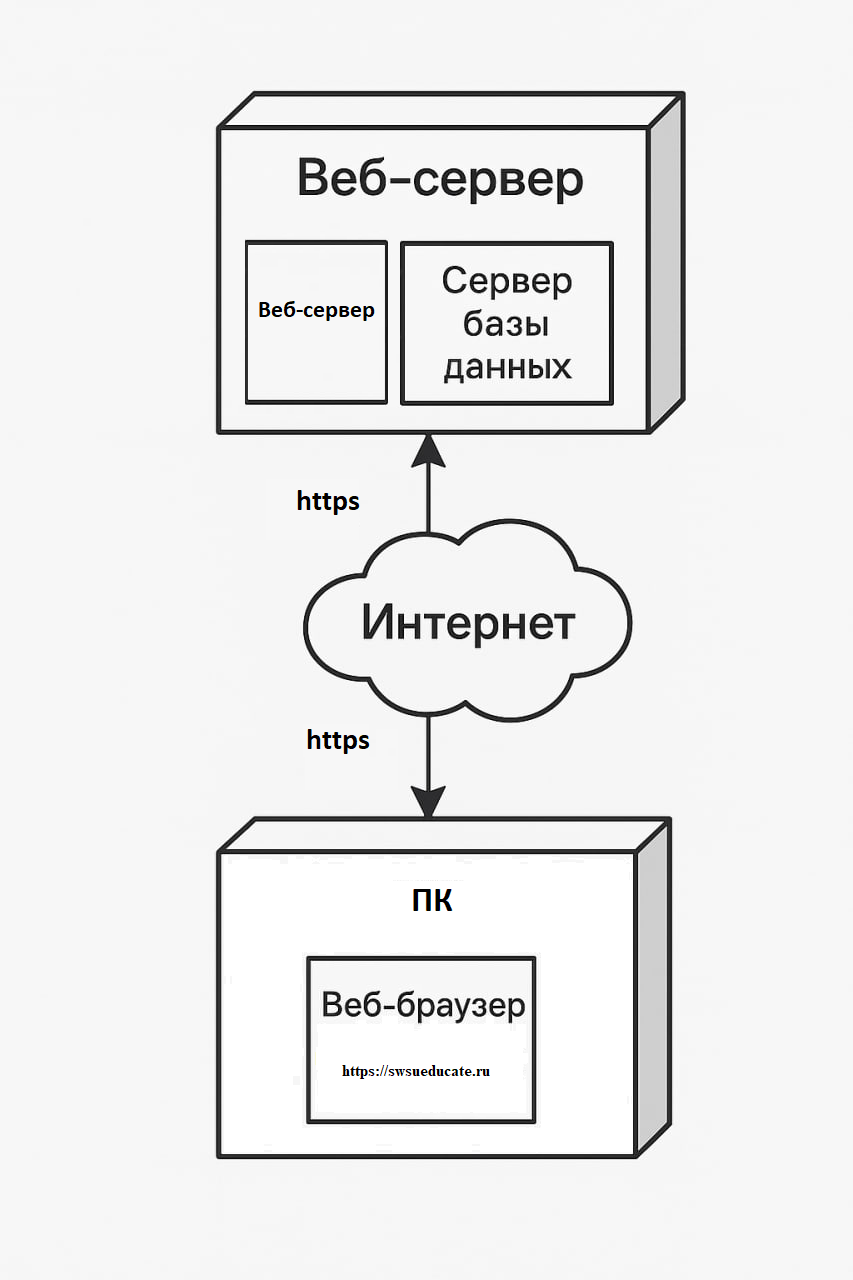
\includegraphics[width=0.57\linewidth]{images/диаграмма2}} 
	\caption{Схема взаимодействия компонентов системы управления обучением}
	\label{system:image}
\end{figure}


\subsection{Отчёты успеваемости}
Одной из причин использования веб-приложения в образовательных целях является удобство формирования отчётов об успеваемости. В системе предусмотрен модуль аналитики, в котором представлена статистическая информация для таких категорий, как прогресс студентов, результаты тестов и активность пользователей. Рассмотрим ключевой отчёт:

\subsubsection{Отчёт по результатам тестов}
Отчёт по результатам тестов представляет собой документ, фиксирующий итоги выполнения тестов студентами за определённый период. Он формирует данные о баллах на момент начала и завершения теста, сведения об общем количестве попыток (attemptnumber), информацию о проходном балле, а также статистику: средний, максимальный и минимальный балл. Пример отчёта представлен на рисунке. 

\begin{figure}[ht]
	\centering
	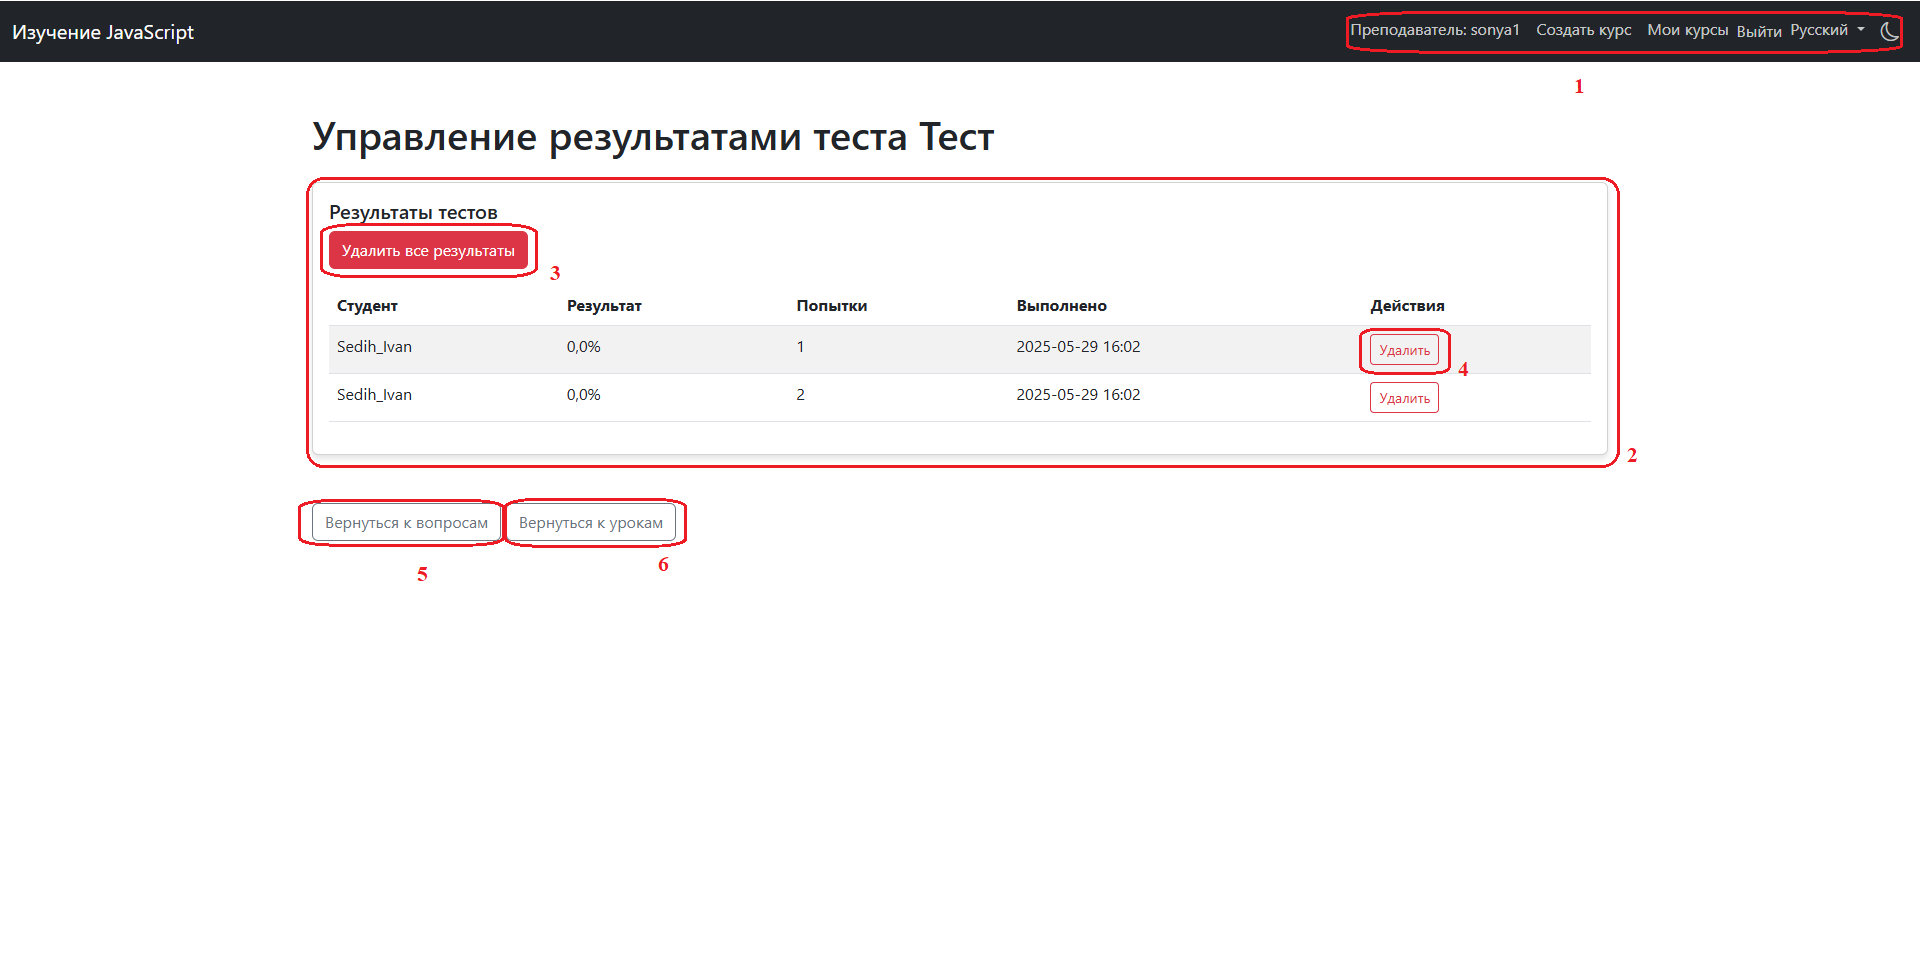
\includegraphics[width=0.7\linewidth]{images/результаты} 
	\caption{Отчёт по результатам тестов}
	\label{zotchet:image}
\end{figure}

Ключевой особенностью данного отчёта является ограничение на количество попыток прохождения теста. Если студент превышает допустимое число попыток, доступ к тесту блокируется, и система уведомляет об этом (messages.error). Каждому отчёту присваивается уникальный идентификатор, исключающий дублирование данных при формировании статистики за определённый период.

Поскольку результаты тестов фиксируются в базе данных SQLite, отчёт не подлежит обнулению или повторному формированию без вмешательства администратора. Данные о результатах автоматически передаются преподавателю через интерфейс (managetestresults), что упрощает анализ. 

Отчёт по результатам тестов необходим: 

\begin{itemize}
	\item студенту для отслеживания своего прогресса и улучшения результатов; 
	\item преподавателю для контроля успеваемости и корректировки учебного плана; 
	\item администратору системы для анализа активности пользователей и проверки корректности работы модуля тестирования.
\end{itemize}

